\section{Модель ресурса сборочной линии}
\indent В процессе создания оперативного плана, для получения корректной оценки времени выполнения операции или набора операций СПП необходимо ввести систему ограничений, которая будет отражать как ресурс\todo{изменить описание, добавить определение, что я понимаю под ресурсом}, участвующий в операции может влиять на её время выполнения.
Это привело к созданию модели ресурсов накладывающей ограничения на выбор операции для расчета ядром имитационного моделирования.
Под ресурсом подразумевается любое устройство,деталь,инструмент или средство,за исключением сырьевого материала и промежуточного продукта, находящиеся в распоряжении предприятия для производства товаров и услуг.
В соответствии с данным определением к ресурсам относятся в том числе и человеческие ресурсы, которые в данной системе не рассматриваются с точки зрения поведения или других аспектов человеческой жизни, а лишь с точки зрения возможности выполнить конкретную задачу.\\
\indent Каждый ресурс представляет из себя структуру данных, которая должна реализовывать три метода:
\begin{itemize}
	\item метод привязки операции к ресурсу;
	\item метод, осуществляющий проверку возможности выполнения данной операции ресурсом;
	\item метод, осуществляющий логику работы и в котором происходит изменение состояния данного ресурса.
\end{itemize}

\indent Под привязкой операции к ресурсу подразумевается добавление операции в очередь на выполнение и, если это первая привязанная для данного продукта операция, то добавление продукта в очередь на распределение. Привязка осуществляется в начале работы системы, что позволяет ресурсам манипулировать ядром имитационного моделирования разрешая или запрещая выбирать привязанные к ним операции для расчета, что может повлечь за собой изменение последовательности выполнения операций и, соответственно, расчетного времени выполнения карты технологического процесса.\\
\indent Проверка производится во время работы системы и именно здесь происходит отбор операций в соответствии с внутренним состоянием ресурса.\\
\indent Логика осуществляется при выборке операции ядром и для каждой вызывается два раза: чтобы отметить состояние ресурса в начале и в конце расчета операции.\\

\todo[inline]{блок-схема ресурсов}

\indent СПП имеет несколько видов ресурсов, одним из которых является ресурс сборочной линии, который описывает несколько однотипных, то есть с одинаковым числом рабочих постов, физических сборочных линий.
Сборочная линия - это способ перемещения заготовки от одного рабочего поста к другому; на каждом посту выполняются закрепленные за ним операции.
Под постами понимаются заготовко-места, оснащенные соответствующим технологическим оборудованием и предназначенными для технического воздействия на заготовку для осуществления фиксированного перечня операций.
Объединение нескольких сборочных линий в одну обуславливается упрощением как взаимодействия с ядром имитационного моделирования так и упрощением управления ресурсом потому как даже в худшем случае (когда все линии будут различны по количеству постов) количество ресурсов будет всегда меньше либо равно количеству физических сборочных линии, а также возможностью инкапсуляции реализации распределения заготовок и связанных с ними операций по сборочным линиям внутри ресурса.

\begin{figure}[h]
	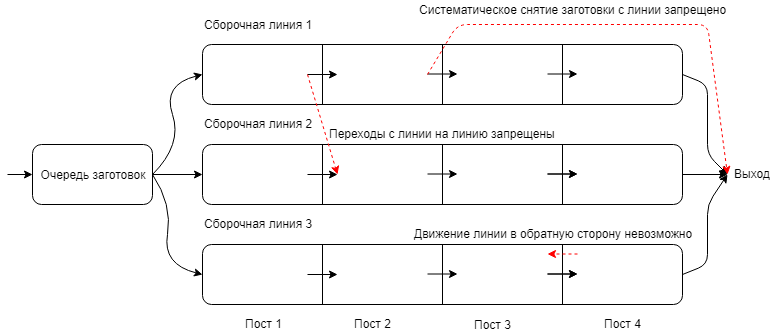
\includegraphics[width=\linewidth]{pics/assemblyMain.png}
	\caption{Схема ресурса с вариантами перемещения заготовки внутри}
	\label{fig:assemblyMain}
	% \centering
\end{figure}
\todo{Добавить цифры к линиям, чтобы ссылаться на конкретные}

\indent Главным предназначением данного ресурса является ограничение перемещения продукции внутри ресурса (см. \ref{fig:assemblyMain}), и моделирование работы физического сборочного конвейера.
С одной стороны ограничивается перемещение между сборочными линиями: к какой продукт был привязан, на той он и останется до окончания выполнения всех операций, относящихся к данному продукту и привязаны к постам данной сборочной линии.
С другой - ограничивается перемещение продукции между рабочими постами: продукт должен двигаться последовательно с поста на пост (см. \ref{fig:assemblyMain}).\\
\indent Одной из ключевых особенностей практически любой сборочной линии является синхронизация передвижения продукции между постами. 
Это означает что такт производства (время,в течение,которого заготовка пребывает на посту) будет равен максимальной временной отметке среди всех постов или другими словами: каждая заготовка сможет сменить пост только после того, как все остальные заготовки будут готовы к смене своих постов.\\
\indent Для реализации необходимого функционала, были введены структуры, описывающие линии, посты, очередь продукции, и проекцию привязки операций к постам линий\todo{что это, пояснение, ссылка на предыдущий рисунок}.
Каждая из линий ресурса характеризуется временем начала текущего рабочего такта сборочной линии, максимальным временем рабочего такта и набором рабочих постов, каждый из которых описывается состоянием (выполняются работы, простаивает, отсутствует продукция на посту), временной меткой данного поста и продукцией, которая на данный момент находится на нем.
Максимальное время отражает какое время работал пост с начала работы системы.
Так как карта технического процесса позволяет, при возможности, производить параллельные операции над заготовкой, то необходимо знать, с какого времени был начат такт, для чего и вводится время начала работы поста.
Время начала текущего рабочего такта показывает время с которого началась работа на текущем посту над текущей заготовкой и для всех постов она равна (из-за синхронизации постов).\\
\todo[inline]{схема постов с флагами}
\indent Проекция привязки операций к постам линий - структура данных необходимая для динамической привязки операций.
Так как во время привязки операции система не может оценить время выполнения продукции и, следовательно, распределив продукты до начала работы может сложиться ситуация, когда одна из линий будет работать намного дольше или наоборот по сравнению с другими линиями, что может привести к простою производству.
Следовательно необходимо, не привязывая операцию к определенной линии, обозначить к какому посту относится операция.
Для этого и была создана данная структура, содержащая то же количество постов что и остальные линии, но не описывающая какую либо физическую сборочную линию, а являющуюся по сути проекцией всех остальных.
Внутри каждого поста данной проекции находится хэш-таблица (структура данных, позволяющая хранить пары (ключ, значение) и выполнять три операции: операцию добавления новой пары, операцию поиска и операцию удаления пары по ключу), в которой ключом является конкретная единица продукции, характеризуемая типом продукции (названием) и серийным номером, а значением - список операций, которые необходимо выполнить над данным продуктом на данном посту.\\
\begin{figure}[h]
	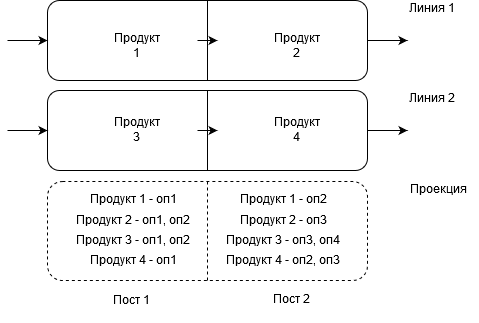
\includegraphics[width=\linewidth]{pics/assemblyBind.png}
	\caption{Схема ресурса с проекцией привязки операций к постам}
	\label{fig:bind}
\end{figure}

\indent Во время выполнения система, для определения возможности выполнения операции опрашивает все линии с целью определения возможности выполнения данной операции и местонахождения продукта:

\begin{itemize}
	\item при отсутствии продукта на всех линиях:
		\begin{enumerate}
			\item[1)] инициируется проверка всех линий на возможность загрузки первого поста (то есть пуст ли он);
			\item[2)] из получившегося списка линий (если количество больше нуля, иначе переход к \ref{itm:point4}\todo{fix reference}) выбирается линия, временная отметка которой является наименьшей среди всех доступных линий;
			\item[3)] возвращается разрешение на выполнение данной операции и временная метка, выбранная на предыдущем шаге;
			\item[\label{itm:point4}{4)}] иначе (количество линий равно нулю) возвращается запрет на выполнение данной операции на текущей итерации.
		\end{enumerate}
	\item если продукт находится на какой-либо линии, то производится опрос проекции:
		\begin{itemize}
			\item \todo{сменить метку}при нахождении нужной операции на посту, на котором находится в данный момент продукт, возвращается разрешение на выполнение и временная метка, с которой может производиться данная операция;
			\item иначе возвращается запрет выполнения.
		\end{itemize}
\end{itemize}

\indent Ядро имитационного моделирования последовательно переберет все доступные на данной итерации и выберет одну из тех, что получили разрешение от всех ресурсов на выполнение.
Если таковых не будет, то система известит о невозможности дальнейшей работы вследствие логической ошибки при задании параметров.
В обратном случае произойдет вызов метода для того, чтобы отметить состояние ресурса в начале выполнения операции.
При этом если продукт не был загружен на линию, то произойдет загрузка продукта на линию с минимальной временной отметкой, иначе произойдет проверка на возможность сдвига линии.\\
\indent Во второй раз метод будет вызван для того, чтобы отметить окончание операции, что означает что данная операция будет удалена из проекции, временная метка поста будет изменена с учетом длительности операции, и, если операций на данном посту для данного продукта не осталось, то состояние поста изменится на 'готов к сдвигу линии' и будет совершена проверка возможности сдвига линии.\\
\indent Сдвиг линии\todo{узнать нет ли определения} - процесс, при котором все посты на сборочной линии передают свою заготовку на следующий пост и принимают заготовку с предыдущего.
Данный процесс единовременен для всех постов, не может быть разделен или проигнорирован каким-либо постом и выполняется после получения от всех постов сигнала о готовности к сдвигу.
При этом происходит синхронизация постов, то есть все посты, и, соответственно вся линия, получают одну временную отметку - сумма предыдущей отметки начала рабочего такта и длительности текущего рабочего такта линии.
С этой отметки начинается отсчет следующего такта.
\todo[inline]{диаграмма ганта по рабочему такту?}
\todo[inline]{описание движения линии}
\todo[inline]{описание синхронизации линии}


% \indent 
% Пояснение сдвигу линии

% \indent Во время работы ядра имитационного моделирования на каждой итерации проверяется наличие привязки ресурсов ко всем доступным для выбора операциям и, при наличии таковых, осуществляется опрос каждого ресурса на то, накладывает ли он какое-либо ограничение на выбор данной операции в текущую итерацию.

% \indent Основной сложностью реализации данного модуля является предложенная система ресурсов, которая является универсальной и позволяет реализовать логику любого ресурса, при этом усложняя реализацию каждого из них.
% Данная компонента является частью (или частной реализацией) модели ресурсов СПП и отражает поведение во времени продуктов на сборочной линии. Основная сложность данной компоненты в необходимости объединения нескольких сборочных линий со схожими параметрами в один ресурс, хранении их состояний, синхронизации между \todo{постами} и распределении \todo{входного потока продуктов} по линиям. Также, сложностью является сама модель ресурса, которая обеспечивает хорошую масштабируемость, но при этом требует времени на понимание и создание модулей.